\documentclass[conference]{IEEEtran}

\usepackage[utf8]{inputenc}
\usepackage[T1]{fontenc}
\usepackage[spanish, es-tabla]{babel}
\usepackage{cite}
\usepackage{amsmath, amssymb, amsfonts}
\usepackage{graphicx}
\usepackage{booktabs}
\usepackage{array}
\usepackage{url}
\usepackage{balance}
\usepackage{hyperref}

\graphicspath{{../resultados/figuras/}}

\hypersetup{
    colorlinks=true,
    linkcolor=black,
    citecolor=black,
    urlcolor=blue
}

\begin{document}

\title{Clasificación Supervisada para el Diagnóstico de Cáncer de Mama mediante Naive Bayes, SVM y Redes Neuronales: Un Enfoque Experimental Reproducible}

\author{
    \IEEEauthorblockN{Raúl Emiliano Sotelo Delgado}
    \IEEEauthorblockA{
        \textit{Ingeniería en Computación} \\
        \textit{Universidad Autónoma del Estado de México, Campus Texcoco} \\
        Texcoco, Estado de México, México \\
        rsotelod001@alumno.uaemex.mx
    }
}

\maketitle

\begin{abstract}
El diagnóstico preciso del cáncer de mama a partir de biopsias por aspiración con aguja fina es fundamental para distinguir tumores malignos de benignos y reducir errores clínicos graves. En este trabajo se aplica el proceso completo de ciencia de datos sobre el conjunto \textit{Breast Cancer Wisconsin (Diagnostic)} del repositorio UCI (569 muestras y 30 variables numéricas). Mediante un sondeo independiente se detectaron ausencia de encabezados, inconsistencias en la columna identificadora, 13 ceros exactos en variables de concavidad pertenecientes a casos benignos, diferencias de escala de hasta seis órdenes de magnitud y 21 pares de variables con correlación superior a 0.90. Se compararon tres modelos supervisados ---Clasificador Bayesiano Ingenuo Gaussiano (\texttt{GaussianNB}), Máquinas de Soporte Vectorial (SVM) y Perceptrón Multicapa (MLP)--- frente a Regresión Logística como referencia, utilizando flujos de trabajo (\textit{pipelines}) con estandarización y validación cruzada estratificada de cinco particiones. En el conjunto de prueba ($n = 114$), MLP alcanzó la mayor sensibilidad (0.9524, con solo dos falsos negativos) y puntaje F1 (0.9639), mientras que SVM obtuvo precisión perfecta (1.0000) y la menor variabilidad entre particiones ($0.9674 \pm 0.0114$).
\end{abstract}

\begin{IEEEkeywords}
Cáncer de mama, clasificación supervisada, análisis exploratorio, Naive Bayes, SVM, perceptrón multicapa, validación cruzada, reproducibilidad.
\end{IEEEkeywords}

\section{Introducción}

El cáncer de mama constituye uno de los problemas de salud pública más relevantes a nivel mundial y una de las principales causas de mortalidad oncológica. Diferenciar correctamente entre un tumor benigno y uno maligno en etapas tempranas resulta determinante para el pronóstico del paciente: un diagnóstico oportuno permite iniciar el tratamiento de inmediato, mientras que una clasificación errónea puede derivar en procedimientos invasivos innecesarios o, en el peor escenario, en dejar sin atención un tumor maligno.

En el ámbito clínico, la biopsia por aspiración con aguja fina (FNA) permite obtener muestras celulares de una masa mamaria y digitalizar imágenes de sus núcleos para medir características geométricas como radio, textura, perímetro, área y concavidad \cite{street1993}. A partir de estas mediciones numéricas es posible entrenar modelos de aprendizaje automático supervisado que sirvan como apoyo objetivo al diagnóstico médico.

Sin embargo, aplicar algoritmos de clasificación sobre conjuntos médicos pequeños (569 pacientes) exige rigor en cada etapa del proceso de ciencia de datos. No basta con reportar un porcentaje alto de exactitud; es indispensable auditar los datos de origen sin asumir que están libres de detalles problemáticos, escalar las variables sin filtrar información del conjunto de prueba, verificar los supuestos estadísticos de cada algoritmo y analizar en qué casos concretos fallan los modelos.

La contribución de este trabajo radica en construir y documentar un flujo experimental completamente reproducible en Python que conecta las técnicas vistas en el curso de Ciencia de Datos con un estudio comparativo riguroso de cuatro algoritmos (Regresión Logística como referencia, Naive Bayes Gaussiano, SVM y Red Neuronal MLP), priorizando la justificación metodológica, la estabilidad estadística y el análisis clínico de los falsos negativos.

\section{Trabajo Relacionado}

El conjunto de datos \textit{Breast Cancer Wisconsin (Diagnostic)} (WDBC) fue creado y publicado por Street, Wolberg y Mangasarian \cite{street1993}, quienes extrajeron diez características morfológicas reales de los núcleos celulares a partir de imágenes digitalizadas de biopsias FNA. Posteriormente, Mangasarian \textit{et al.} \cite{mangasarian1995} emplearon programación lineal para construir planos separadores sobre estas variables, logrando tasas de exactitud cercanas al 97.5\% y evidenciando que el problema presenta una separabilidad casi lineal en el espacio de atributos.

A partir de la formulación formal de las Máquinas de Soporte Vectorial por Cortes y Vapnik \cite{cortes1995}, SVM se consolidó como uno de los clasificadores más efectivos para conjuntos tabulares de tamaño moderado gracias a la maximización del margen y al control de complejidad mediante regularización. En el diagnóstico de cáncer de mama, Akay \cite{akay2009} combinó SVM con selección de características, comprobando su alta precisión incluso frente a la redundancia natural de las mediciones celulares.

En paralelo, las redes neuronales multicapa entrenadas por retropropagación, descritas por Rumelhart, Hinton y Williams \cite{rumelhart1986}, han sido ampliamente utilizadas para modelar fronteras no lineales; no obstante, cuando el tamaño muestral es reducido requieren arquitecturas compactas y mecanismos explícitos de regularización para no sobreajustar. Por su parte, el clasificador Naive Bayes ofrece una alternativa probabilística rápida; Rish \cite{rish2001} demostró que aunque puede mantener un rendimiento aceptable bajo dependencias entre variables, la violación del supuesto de independencia condicional degrada su desempeño discriminativo y la calibración de sus probabilidades.

Finalmente, la biblioteca Scikit-Learn \cite{pedregosa2011} estandarizó el uso de objetos \texttt{Pipeline} y validación cruzada estratificada, herramientas que permiten reproducir experimentos y prevenir la fuga de datos durante el ajuste de hiperparámetros.

\section{Metodología}

\subsection{Origen de los Datos y Sondeo Independiente de Errores}

Se trabajó con el conjunto de datos \textit{Breast Cancer Wisconsin (Diagnostic)} del repositorio UCI \cite{street1993}, compuesto por $N = 569$ muestras y 30 variables numéricas continuas. Para cada núcleo celular se calculan diez atributos base (radio, textura, perímetro, área, suavidad, compacidad, concavidad, puntos cóncavos, simetría y dimensión fractal) bajo tres estadísticos: promedio (\textit{mean}), error estándar (\textit{se}) y el promedio de los tres valores más grandes (\textit{worst}).

Aunque la documentación oficial (\texttt{wdbc.names}) señala que la base de datos no contiene valores faltantes, se decidió no confiar ciegamente y desarrollar un script independiente (\texttt{src/01\_sondeo\_errores.py}), retomando los procedimientos de exploración vistos en clase en los cuadernos \texttt{Clase 3-4 EDA/Untitled.ipynb} y \texttt{Tratamiento de complejidad de datos/04\_PreparacionDatos.ipynb}. Al ejecutar este sondeo se confirmó que existen 0 valores nulos y 0 filas duplicadas exactas, pero se identificaron siete hallazgos clave que condicionan el preprocesamiento:

\begin{enumerate}
    \item \textbf{Ausencia de encabezados:} El archivo \texttt{wdbc.data} comienza directamente con el primer paciente. Utilizar \texttt{pd.read\_csv()} de forma estándar provocaría que Python interpretara el primer registro como los nombres de las columnas. Se resolvió cargando el archivo con \texttt{header=None} y asignando manualmente las 32 etiquetas conforme a la sección 7 de \texttt{wdbc.names}.
    \item \textbf{Columna identificadora irrelevante:} La columna \texttt{id} presenta longitudes inconsistentes (de 4 a 9 dígitos) y carece de valor biológico predictivo, por lo que se eliminó directamente mediante \texttt{df.drop(columns=['id'])}, tal como se practicó en \texttt{04\_PreparacionDatos.ipynb}.
    \item \textbf{Codificación de la variable objetivo:} Las etiquetas de diagnóstico vienen en formato de texto (\texttt{M} y \texttt{B}). Se codificaron a valores binarios numéricos asignando \texttt{1} a Maligno y \texttt{0} a Benigno, de modo que la sensibilidad (\textit{recall}) mida directamente la capacidad de detectar casos de cáncer.
    \item \textbf{Ceros exactos en concavidad:} Se detectaron exactamente 13 ceros en \texttt{mean\_concavity}, \texttt{mean\_concave\_points}, \texttt{worst\_concavity} y \texttt{worst\_concave\_points}. Al cruzarlos con el diagnóstico, se comprobó que el 100\% (13 de 13) corresponde a tumores benignos con contornos celulares completamente lisos; no son datos faltantes encubiertos, aunque generan distribuciones sesgadas a la derecha.
    \item \textbf{Diferencia extrema de escalas:} Existen variaciones de hasta seis órdenes de magnitud entre atributos, desde \texttt{se\_smoothness} (mínimo $0.001713$, máximo $0.0311$) hasta \texttt{worst\_area} (mínimo $185.2$, máximo $4254.0$). Sin estandarización, las variables de mayor magnitud dominarían las distancias en SVM y desestabilizarían el gradiente en la red neuronal.
    \item \textbf{Multicolinealidad severa:} Se detectaron 21 pares de variables con correlación de Pearson superior a $0.90$, destacando \texttt{mean\_radius} frente a \texttt{mean\_perimeter} ($r = 0.9979$), \texttt{worst\_radius} frente a \texttt{worst\_perimeter} ($r = 0.9937$), \texttt{mean\_radius} frente a \texttt{mean\_area} ($r = 0.9874$) y \texttt{mean\_radius} frente a \texttt{worst\_radius} ($r = 0.9695$). Dado que \textit{mean} y \textit{worst} miden el mismo fenómeno físico y el área/perímetro dependen geométricamente del radio, se viola directamente el supuesto de independencia de Naive Bayes.
    \item \textbf{Casos atípicos y casos frontera:} Se hallaron 2 pacientes malignos donde \texttt{mean\_radius} y \texttt{worst\_radius} son idénticos (ID \texttt{855133} con $14.99$ y ID \texttt{8810703} con $28.11$), además de 6 tumores malignos pequeños (\texttt{mean\_radius} $< 12$) y 6 tumores benignos grandes (\texttt{mean\_radius} $> 16$), que conforman zonas de traslape propensas a error.
\end{enumerate}

\subsection{Análisis Exploratorio de Datos y Preprocesamiento}

Con base en el sondeo anterior, se implementó el script \texttt{src/02\_preparacion\_y\_eda.py} empleando \texttt{pandas}, \texttt{matplotlib}, \texttt{seaborn} y \texttt{scikit-learn} para generar tres visualizaciones interpretadas (Figs.~\ref{fig:clases} a~\ref{fig:correlacion}):

\begin{itemize}
    \item La Fig.~\ref{fig:clases} muestra la distribución de clases: 357 muestras benignas (62.74\%) y 212 malignas (37.26\%). Al existir un desbalance moderado, se utilizó muestreo estratificado (\texttt{stratify=y}) en todas las divisiones para preservar esta proporción.
    \item La Fig.~\ref{fig:distribucion} compara las curvas de densidad de cuatro atributos morfológicos clave (\texttt{mean\_radius}, \texttt{mean\_texture}, \texttt{mean\_perimeter} y \texttt{mean\_area}), evidenciando que los tumores malignos desplazan sus distribuciones hacia valores mayores, pero existe una franja intermedia de traslape (especialmente entre radios de 12 y 16) donde ambos diagnósticos coinciden.
    \item La Fig.~\ref{fig:correlacion} presenta el mapa de calor de correlaciones de Pearson para las diez variables \textit{mean}, confirmando visualmente los bloques de alta multicolinealidad entre radio, perímetro, área, concavidad y puntos cóncavos.
\end{itemize}

\begin{figure}[t]
    \centering
    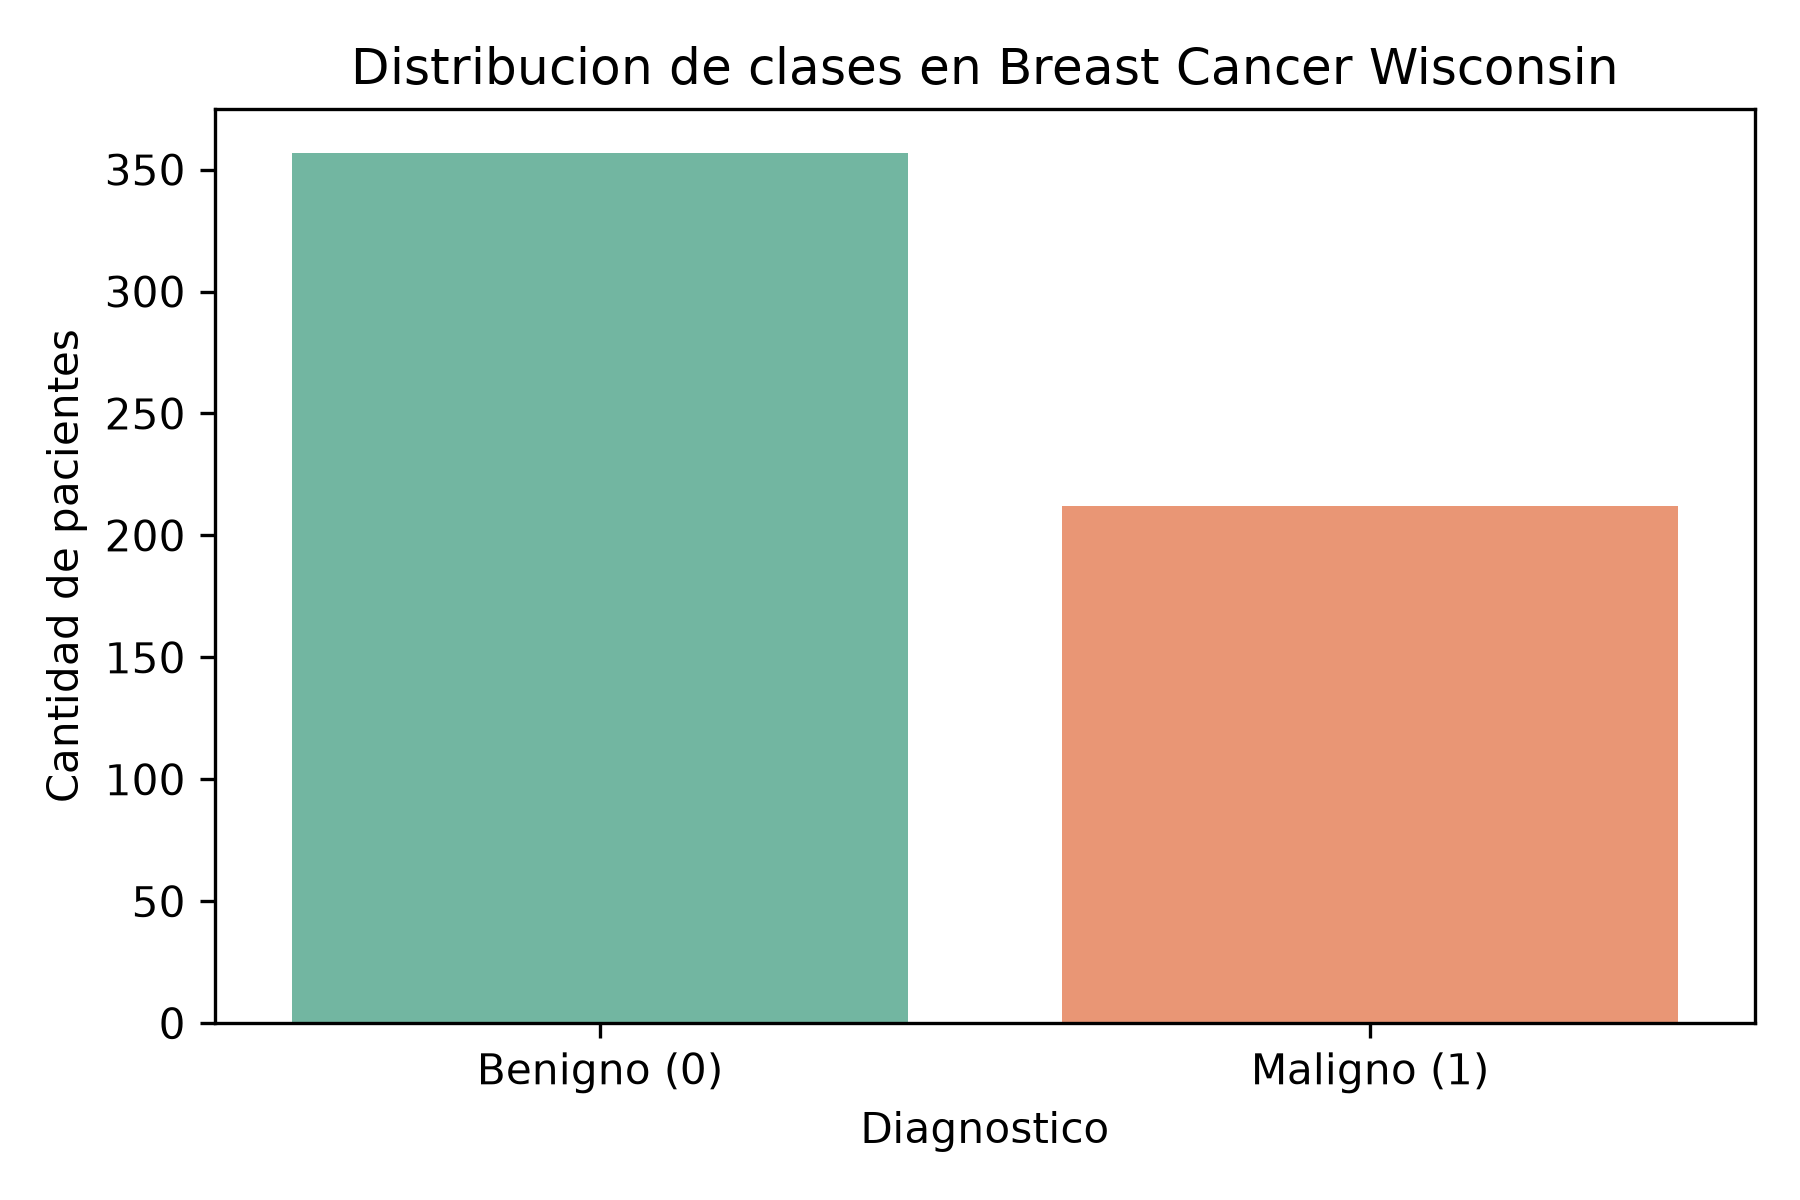
\includegraphics[width=0.88\columnwidth]{01_distribucion_clases}
    \caption{Distribución de clases en Breast Cancer Wisconsin: 357 casos benignos (62.74\%) y 212 malignos (37.26\%).}
    \label{fig:clases}
\end{figure}

\begin{figure}[t]
    \centering
    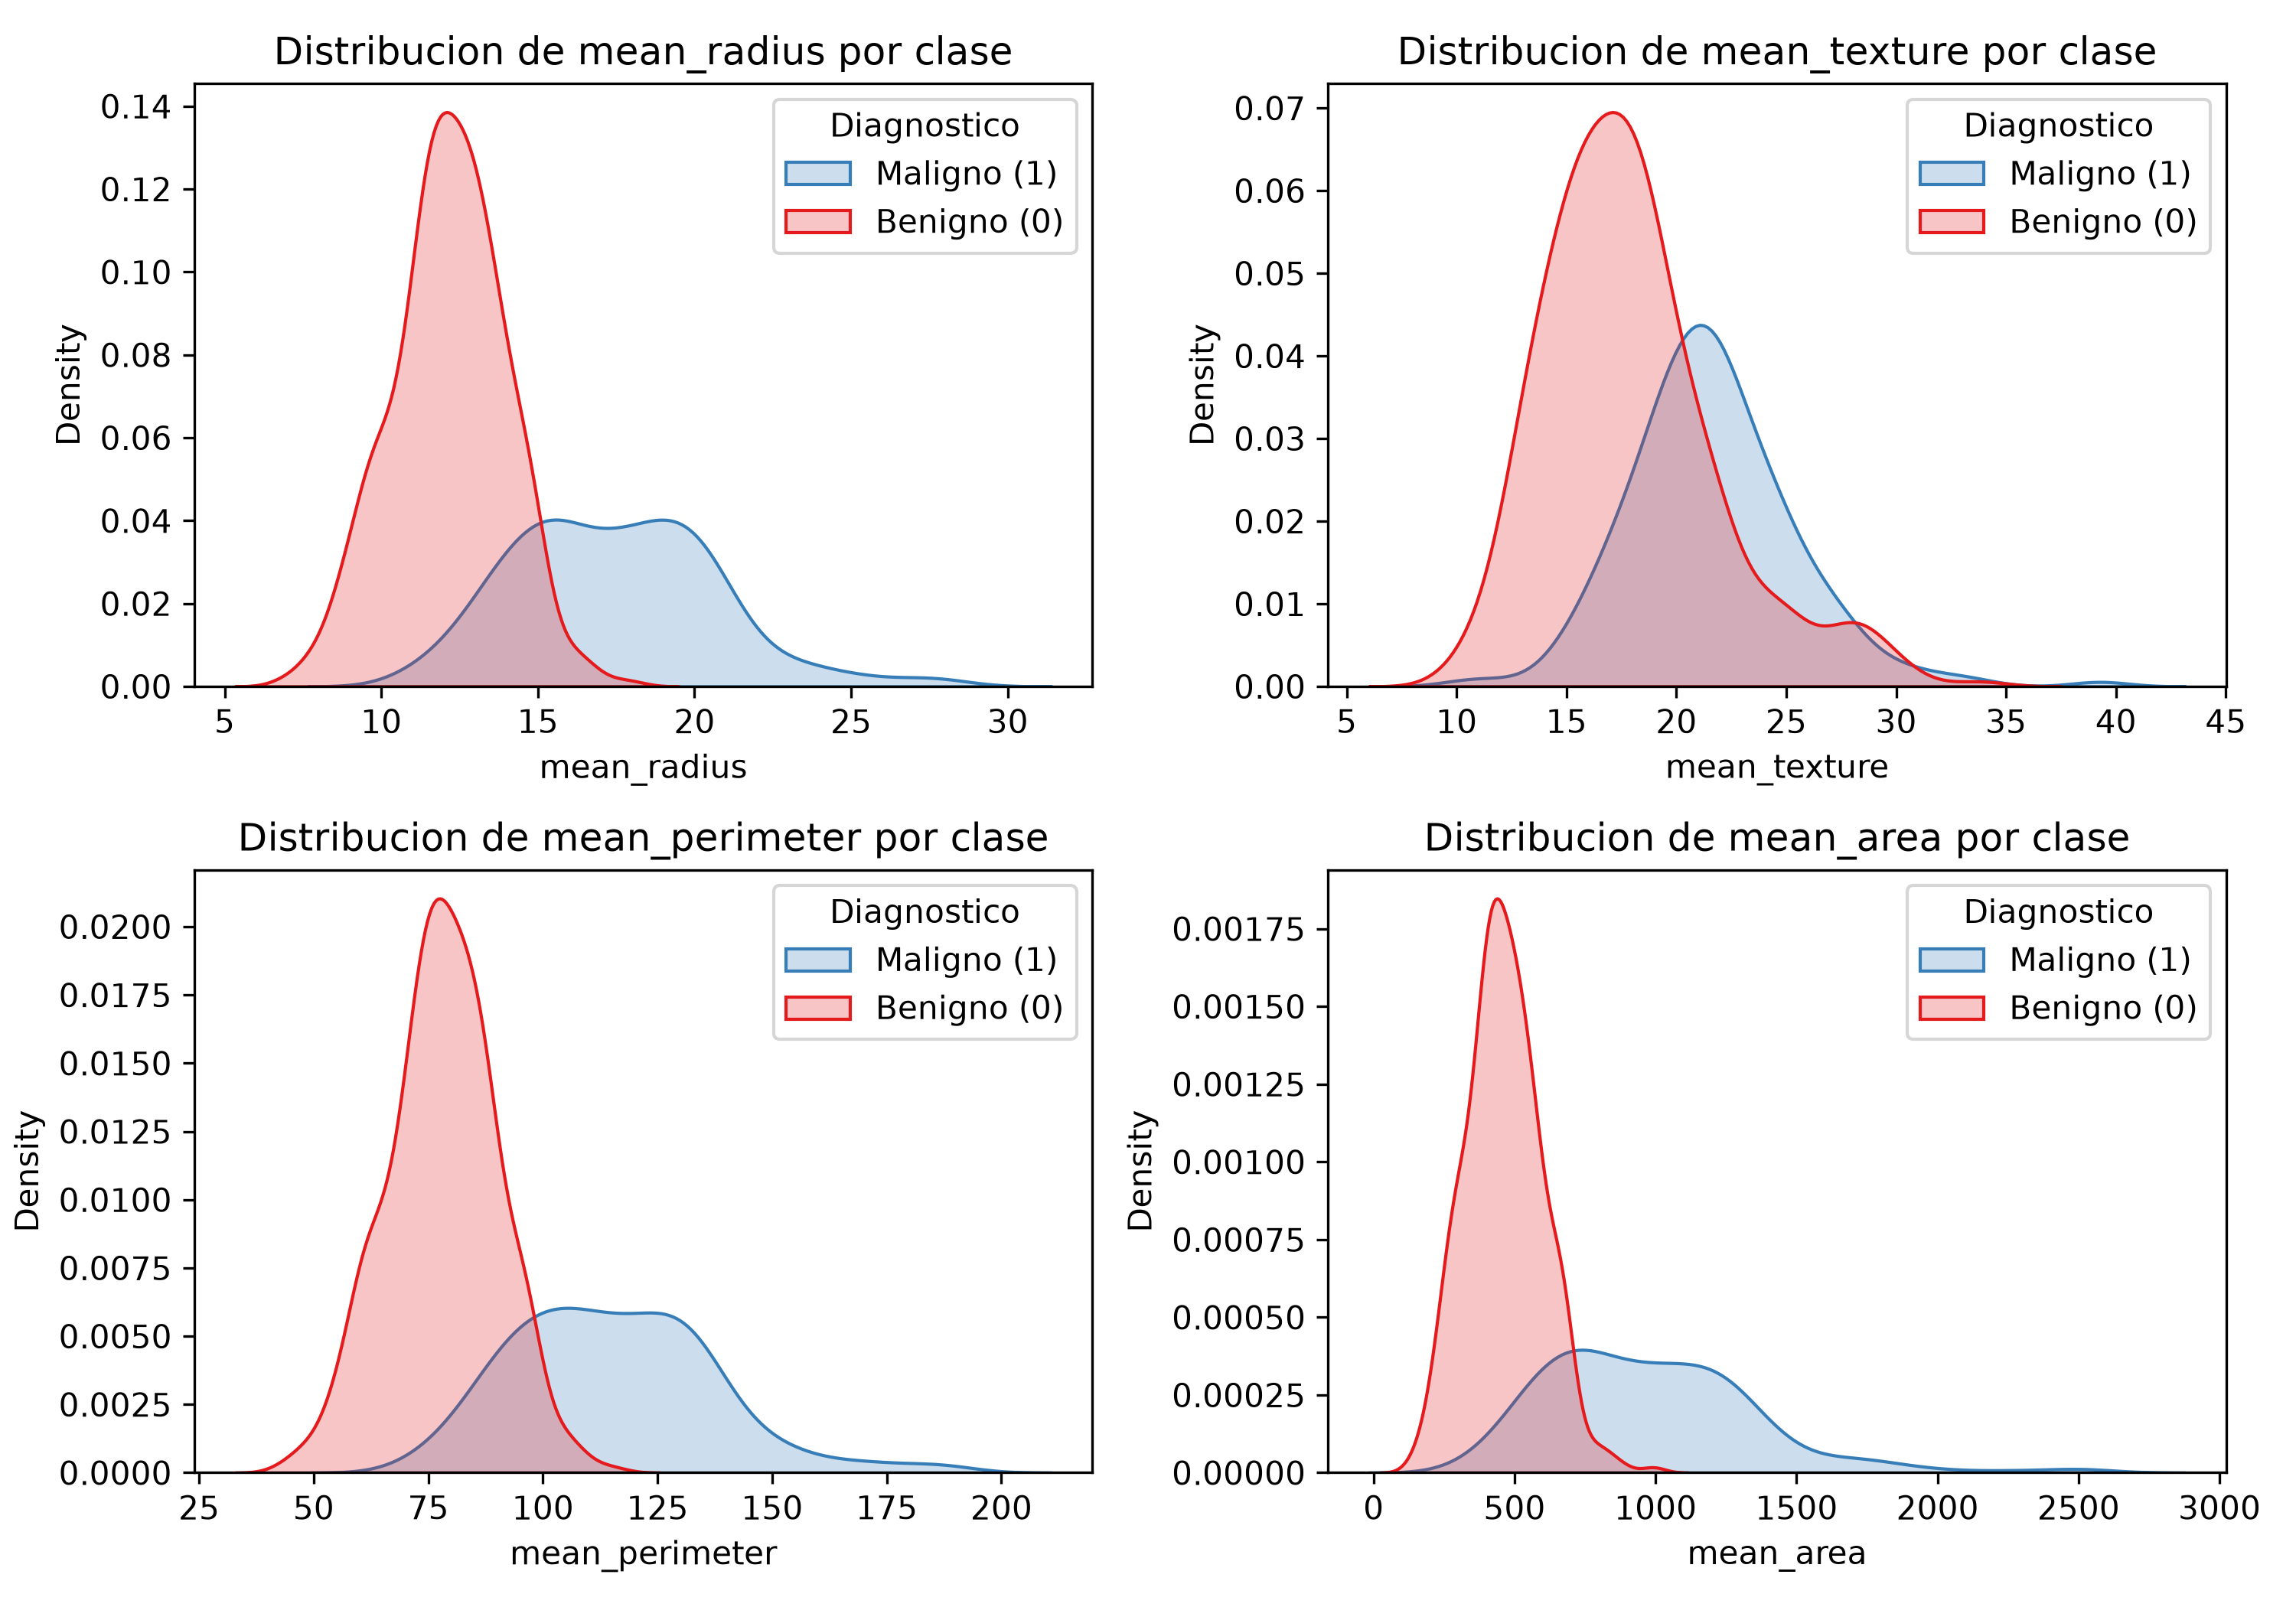
\includegraphics[width=\columnwidth]{02_distribucion_variables}
    \caption{Curvas de densidad por clase para las variables \texttt{mean\_radius}, \texttt{mean\_texture}, \texttt{mean\_perimeter} y \texttt{mean\_area}, mostrando la zona de traslape.}
    \label{fig:distribucion}
\end{figure}

\begin{figure}[t]
    \centering
    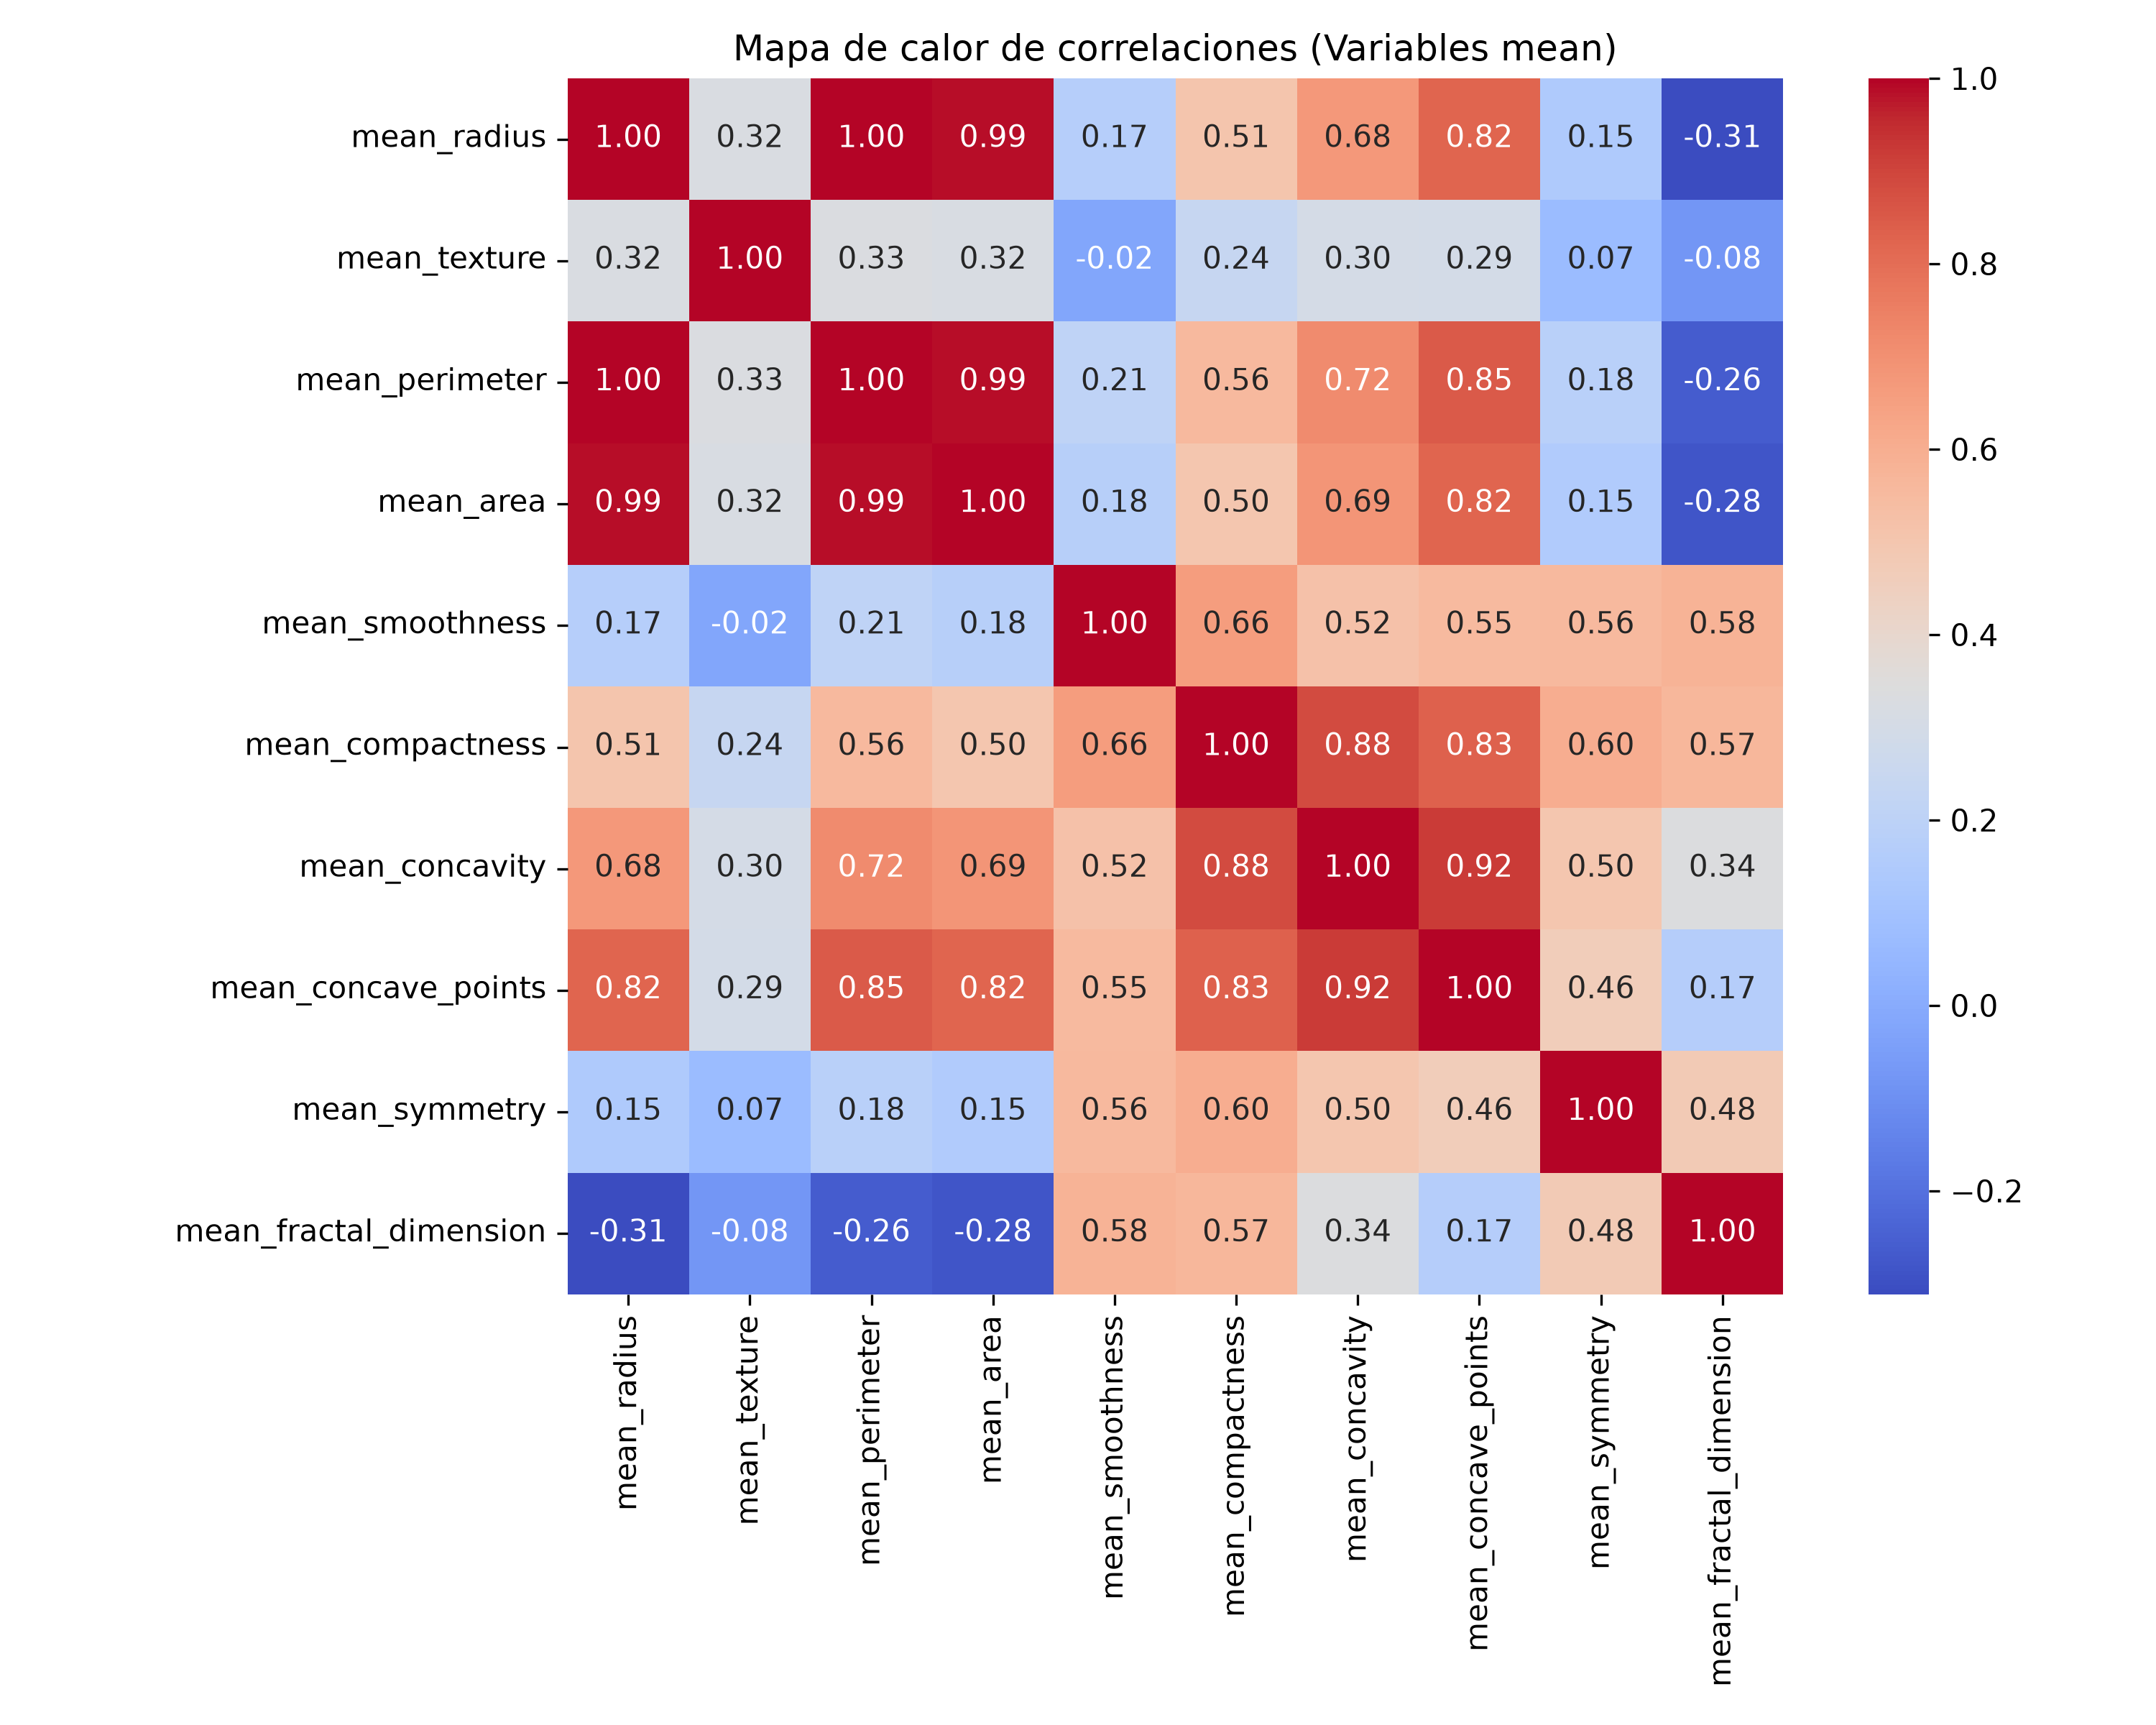
\includegraphics[width=\columnwidth]{03_correlacion_mean}
    \caption{Mapa de calor de correlaciones de Pearson para las diez variables \textit{mean}, evidenciando la multicolinealidad severa.}
    \label{fig:correlacion}
\end{figure}

Para garantizar reproducibilidad absoluta se fijó la semilla \texttt{RANDOM\_STATE = 42}. En el módulo independiente de preparación (\texttt{02\_preparacion\_y\_eda.py}) se generaron particiones estratificadas de entrenamiento (398 muestras, 70\%), validación (85 muestras, 15\%) y prueba (86 muestras, 15\%), ajustando \texttt{StandardScaler} exclusivamente con entrenamiento. Posteriormente, para el ajuste formal de hiperparámetros en \texttt{src/03\_modelos\_y\_evaluacion.py}, se reservó un 20\% intacto para prueba ($n = 114$: 72 benignos y 42 malignos) y sobre el 80\% restante ($n = 455$) se encapsuló \texttt{StandardScaler} dentro de un \texttt{Pipeline} evaluado con validación cruzada estratificada de 5 particiones (\textit{5-Fold Stratified CV}). De esta manera, la media y desviación estándar se recalculan únicamente sobre el subconjunto de entrenamiento de cada fold, eliminando cualquier fuga de datos (\textit{data leakage}).

\subsection{Selección y Justificación de Modelos}

En los materiales vistos en clase se trabajaron el clasificador bayesiano (\texttt{NAIVELLES.ipynb}) y las redes neuronales (\texttt{07\_RedesNeuronales.ipynb}). Para cumplir con los requisitos del estudio y contar con una comparación sólida, se implementaron cuatro algoritmos:

\begin{enumerate}
    \item \textbf{Regresión Logística (Modelo de Referencia):} Se eligió como línea base para verificar si un modelo lineal simple resuelve de forma efectiva el problema antes de recurrir a arquitecturas complejas. Calcula una combinación lineal ponderada de las variables y aplica la función sigmoide para estimar la probabilidad de malignidad.
    \item \textbf{Clasificador Bayesiano (\texttt{GaussianNB}):} Seleccionado por ser la variante adecuada para variables numéricas continuas, siguiendo la base vista en \texttt{NAIVELLES.ipynb}. Aplica el teorema de Bayes asumiendo distribución normal por clase e independencia condicional entre atributos; como comprobó la Fig.~\ref{fig:correlacion}, este segundo supuesto no se cumple en el dataset.
    \item \textbf{Máquina de Soporte Vectorial (SVM):} Incorporada por su desempeño sobresaliente en conjuntos pequeños y de alta dimensión. Busca el hiperplano que maximiza el margen entre clases \cite{cortes1995}. Se probaron el kernel lineal y el kernel RBF ajustando $C$ (penalización de errores en el margen) y $\gamma$ (alcance de influencia de cada muestra).
    \item \textbf{Red Neuronal (\texttt{MLPClassifier}):} Basada en el perceptrón multicapa visto en \texttt{07\_RedesNeuronales.ipynb}, formado por capas de neuronas con transformaciones lineales y funciones de activación no lineales (\texttt{relu} y \texttt{tanh}). Al disponer de solo 455 muestras de entrenamiento, se justificó usar arquitecturas compactas de una y dos capas ocultas ---$(32,)$, $(64, 32)$ y $(32, 16)$--- combinadas con regularización $L_2$ (\texttt{alpha}) y detención temprana (\texttt{early\_stopping=True}) para evitar sobreajuste.
\end{enumerate}

El ajuste de hiperparámetros se realizó mediante búsqueda en malla (\texttt{GridSearchCV}) con validación cruzada estratificada de 5 folds, optimizando el puntaje F1 para equilibrar precisión y sensibilidad. El espacio de búsqueda evaluado se detalla en la Tabla~\ref{tab:espacio_busqueda}.

\begin{table}[t]
    \centering
    \caption{Espacio de Búsqueda de Hiperparámetros en GridSearchCV (5-Fold)}
    \label{tab:espacio_busqueda}
    \renewcommand{\arraystretch}{1.2}
    \begin{tabular}{@{}p{2.3cm}p{5.7cm}@{}}
        \toprule
        \textbf{Modelo} & \textbf{Espacio de Hiperparámetros Probado} \\
        \midrule
        Regresión Logística & $C \in \{0.01, 0.1, 1, 10, 100\}$ \\
        \addlinespace
        Naive Bayes (GaussianNB) & \texttt{var\_smoothing} $\in \{10^{-9}, 10^{-8}, 10^{-7}, 10^{-6}\}$ \\
        \addlinespace
        SVM & Lineal: $C \in \{0.1, 1, 10, 100\}$ \\
            & RBF: $C \in \{0.1, 1, 10, 100\}$, $\gamma \in \{\text{scale}, 0.01, 0.001\}$ \\
        \addlinespace
        Red Neuronal (MLP) & Capas: $\{(32,), (64,32), (32,16)\}$ \\
                           & Activación: $\{\text{relu}, \text{tanh}\}$ \\
                           & $\alpha \in \{10^{-4}, 10^{-3}, 10^{-2}\}$, \texttt{early\_stopping=True} \\
        \bottomrule
    \end{tabular}
\end{table}

\section{Experimentos y Resultados}

\subsection{Comparación de Desempeño y Variabilidad}

Una vez ejecutado \texttt{src/03\_modelos\_y\_evaluacion.py}, se evaluó la variabilidad (media y desviación estándar del puntaje F1 a través de los 5 folds) y se midió el rendimiento final de cada modelo ganador sobre el conjunto de prueba independiente ($n = 114$). La Tabla~\ref{tab:resultados} concentra todas las métricas obtenidas.

En validación cruzada, SVM con kernel RBF ($C = 10$, $\gamma = \text{scale}$) alcanzó el mayor puntaje F1 promedio y la menor desviación estándar ($0.9674 \pm 0.0114$), seguido muy de cerca por la Regresión Logística ($0.9640 \pm 0.0207$). En el conjunto de prueba independiente, tanto SVM como la Red Neuronal MLP empataron en la mayor exactitud ($0.9737$, equivalente a 111 aciertos de 114); sin embargo, MLP logró el mayor puntaje F1 ($0.9639$) y la mayor sensibilidad ($0.9524$), mientras que SVM alcanzó una precisión perfecta ($1.0000$, cero falsos positivos). Por su parte, la Regresión Logística obtuvo el área bajo la curva ROC más alta ($0.9960$), seguida inmediatamente por MLP ($0.9954$). En contraste, Naive Bayes quedó claramente rezagado tanto en validación cruzada ($0.9170 \pm 0.0342$) como en prueba (F1 de $0.8889$ y sensibilidad de $0.8571$).

\begin{table*}[t]
    \centering
    \caption{Resultados Comparativos en Validación Cruzada (5-Fold) y Conjunto de Prueba ($n = 114$)}
    \label{tab:resultados}
    \renewcommand{\arraystretch}{1.25}
    \begin{tabular}{@{}lccccccc@{}}
        \toprule
        \textbf{Modelo} & \textbf{Mejores Hiperparámetros} & \textbf{CV F1 (Media $\pm$ DE)} & \textbf{Accuracy} & \textbf{Precision} & \textbf{Recall} & \textbf{F1} & \textbf{ROC-AUC} \\
        \midrule
        Regresión Logística (Ref) & \texttt{C=1} & $0.9640 \pm 0.0207$ & 0.9649 & 0.9750 & 0.9286 & 0.9512 & \textbf{0.9960} \\
        Naive Bayes (GaussianNB)  & \texttt{var\_s=1e-9} & $0.9170 \pm 0.0342$ & 0.9211 & 0.9231 & 0.8571 & 0.8889 & 0.9891 \\
        SVM                       & \texttt{rbf, C=10, scale} & $\mathbf{0.9674 \pm 0.0114}$ & \textbf{0.9737} & \textbf{1.0000} & 0.9286 & 0.9630 & 0.9927 \\
        Red Neuronal (MLP)        & \texttt{(32,), tanh, 1e-4} & $0.9388 \pm 0.0140$ & \textbf{0.9737} & 0.9756 & \textbf{0.9524} & \textbf{0.9639} & 0.9954 \\
        \bottomrule
    \end{tabular}
\end{table*}

Las matrices de confusión del conjunto de prueba se ilustran en la Fig.~\ref{fig:confusion}, detallando el balance exacto de verdaderos positivos, verdaderos negativos, falsos positivos y falsos negativos. Complementariamente, las curvas ROC (Fig.~\ref{fig:roc}) y las curvas Precisión-Recall (Fig.~\ref{fig:pr}) confirman que Regresión Logística, SVM y MLP mantienen un área bajo la curva cercana a la unidad (con precisión promedio $\text{AP} = 0.99$), mientras que Naive Bayes cae a $\text{AP} = 0.98$ al degradarse su precisión en niveles altos de sensibilidad.

\begin{figure}[t]
    \centering
    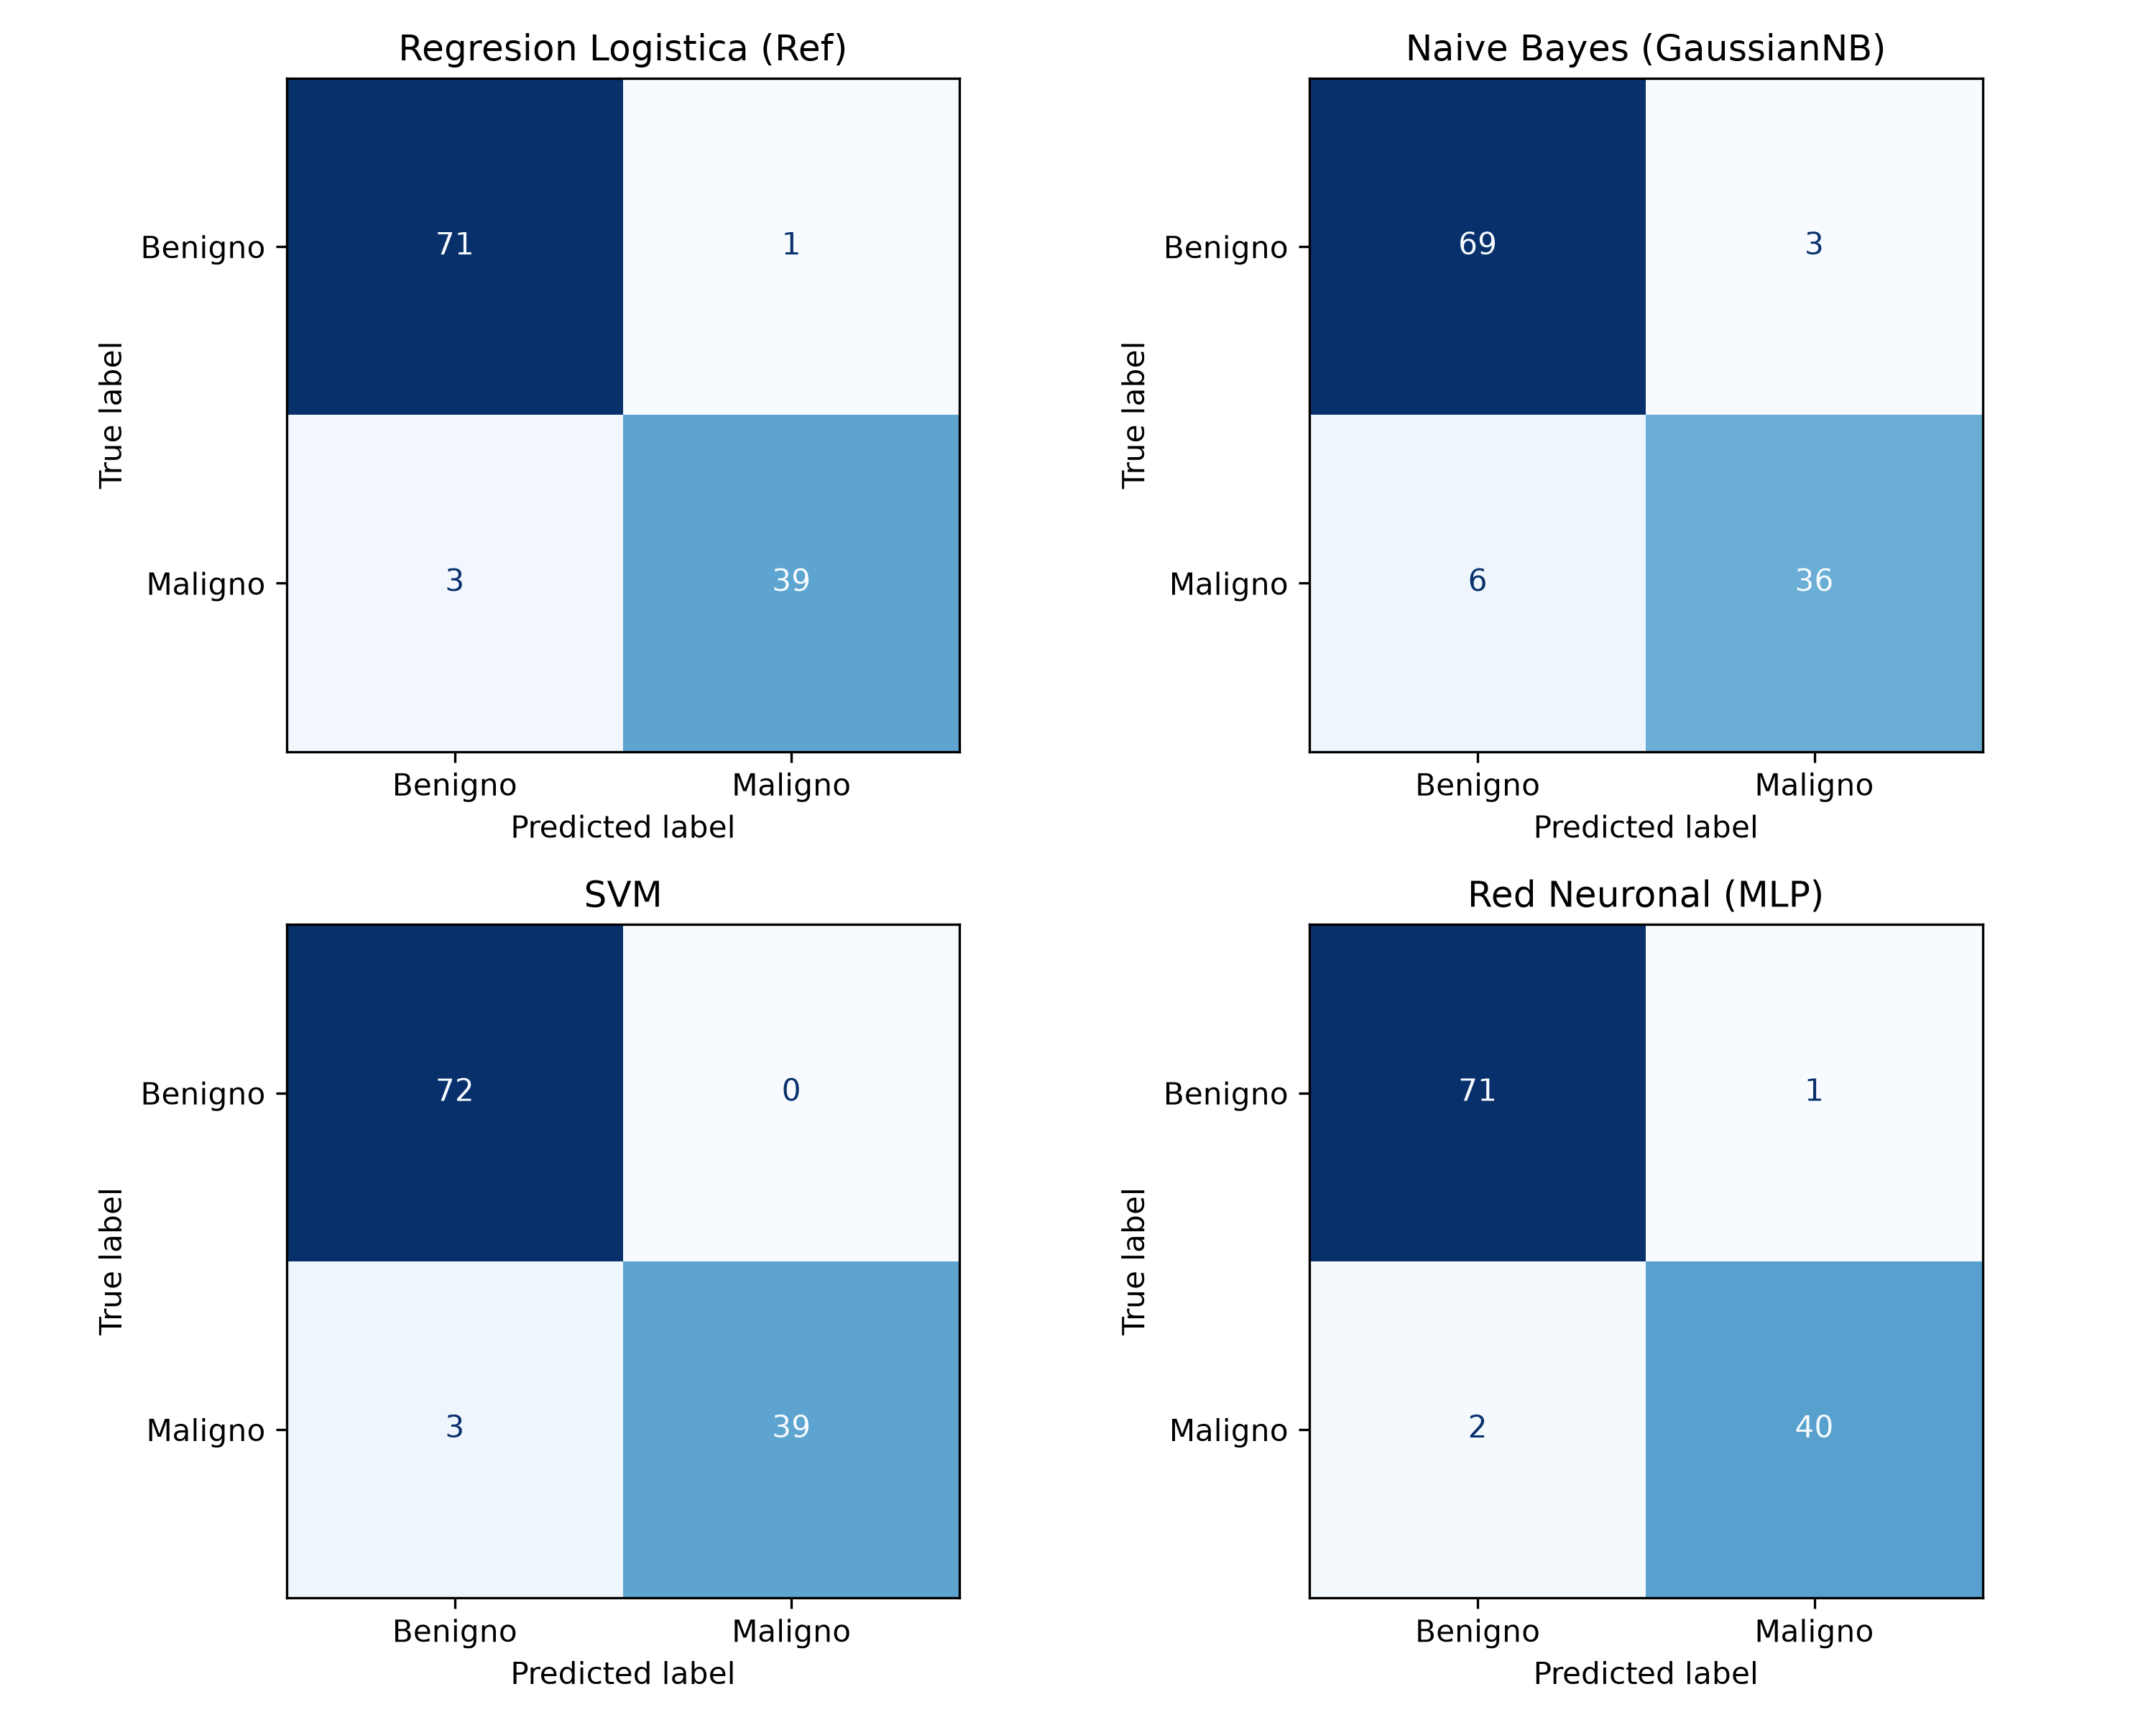
\includegraphics[width=\columnwidth]{04_matrices_confusion}
    \caption{Matrices de confusión de los cuatro clasificadores evaluados sobre el conjunto de prueba independiente ($n = 114$).}
    \label{fig:confusion}
\end{figure}

\begin{figure}[t]
    \centering
    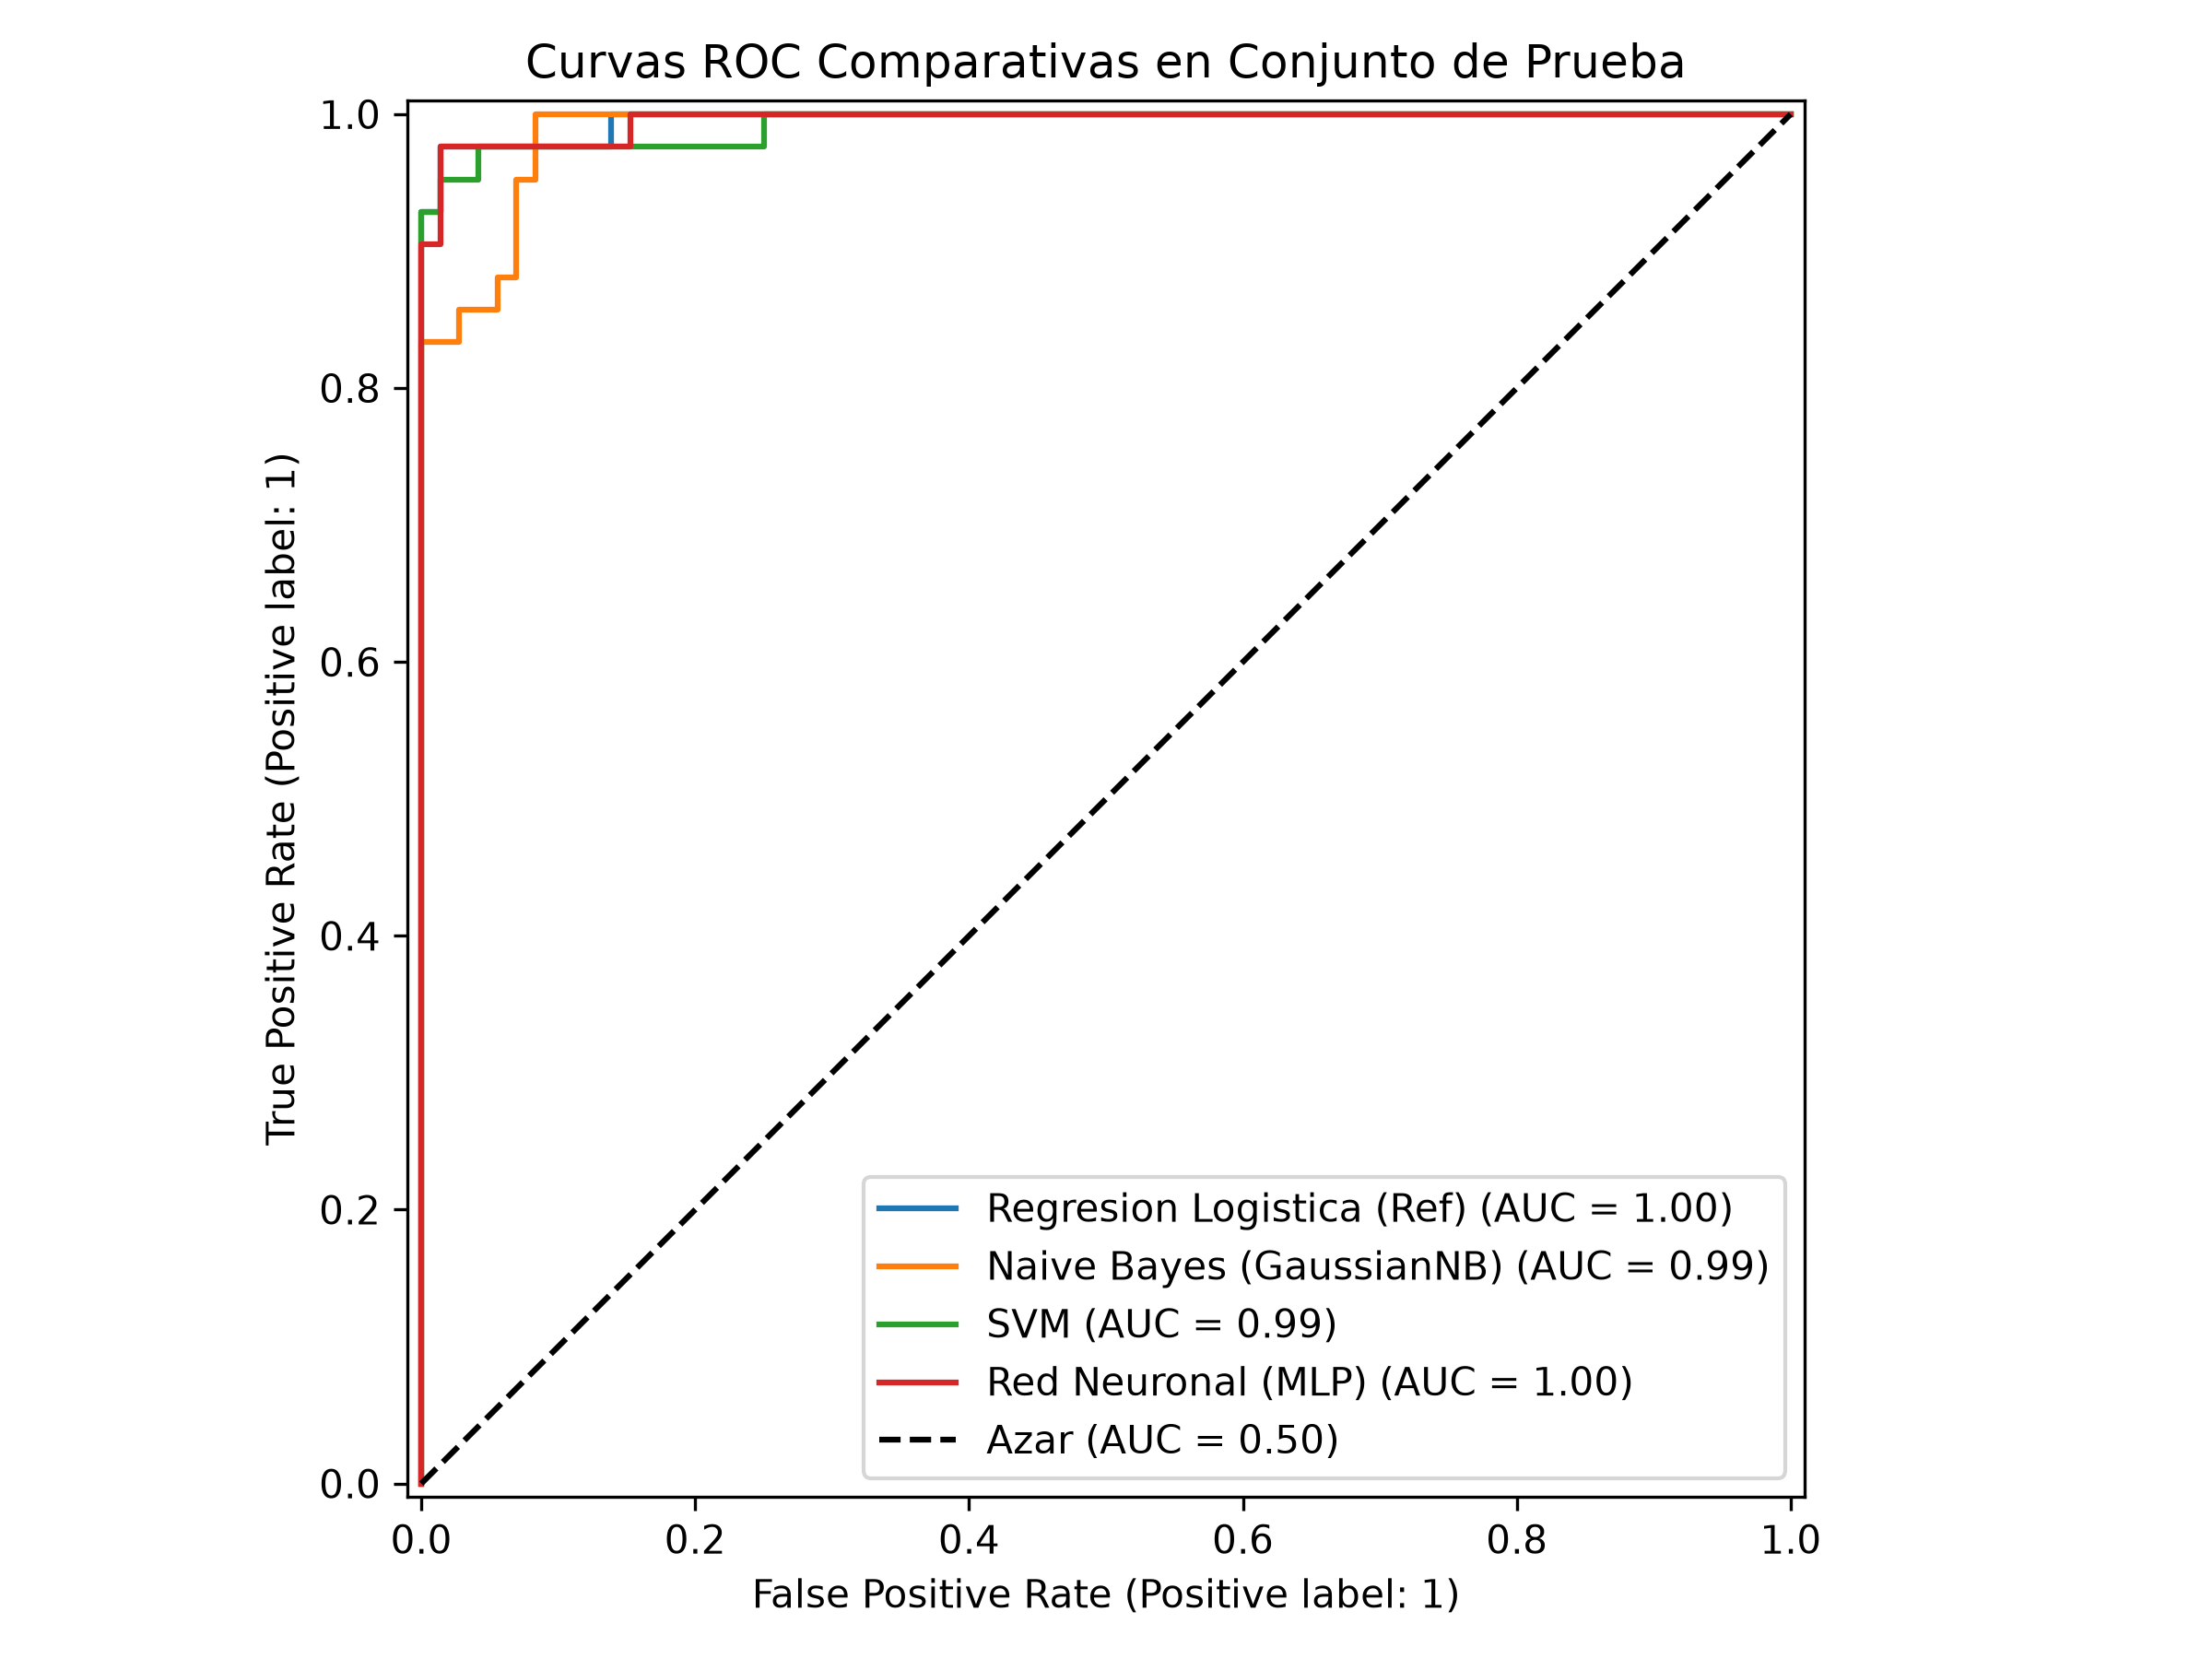
\includegraphics[width=0.92\columnwidth]{05_curvas_roc}
    \caption{Curvas ROC comparativas sobre el conjunto de prueba independiente.}
    \label{fig:roc}
\end{figure}

\begin{figure}[t]
    \centering
    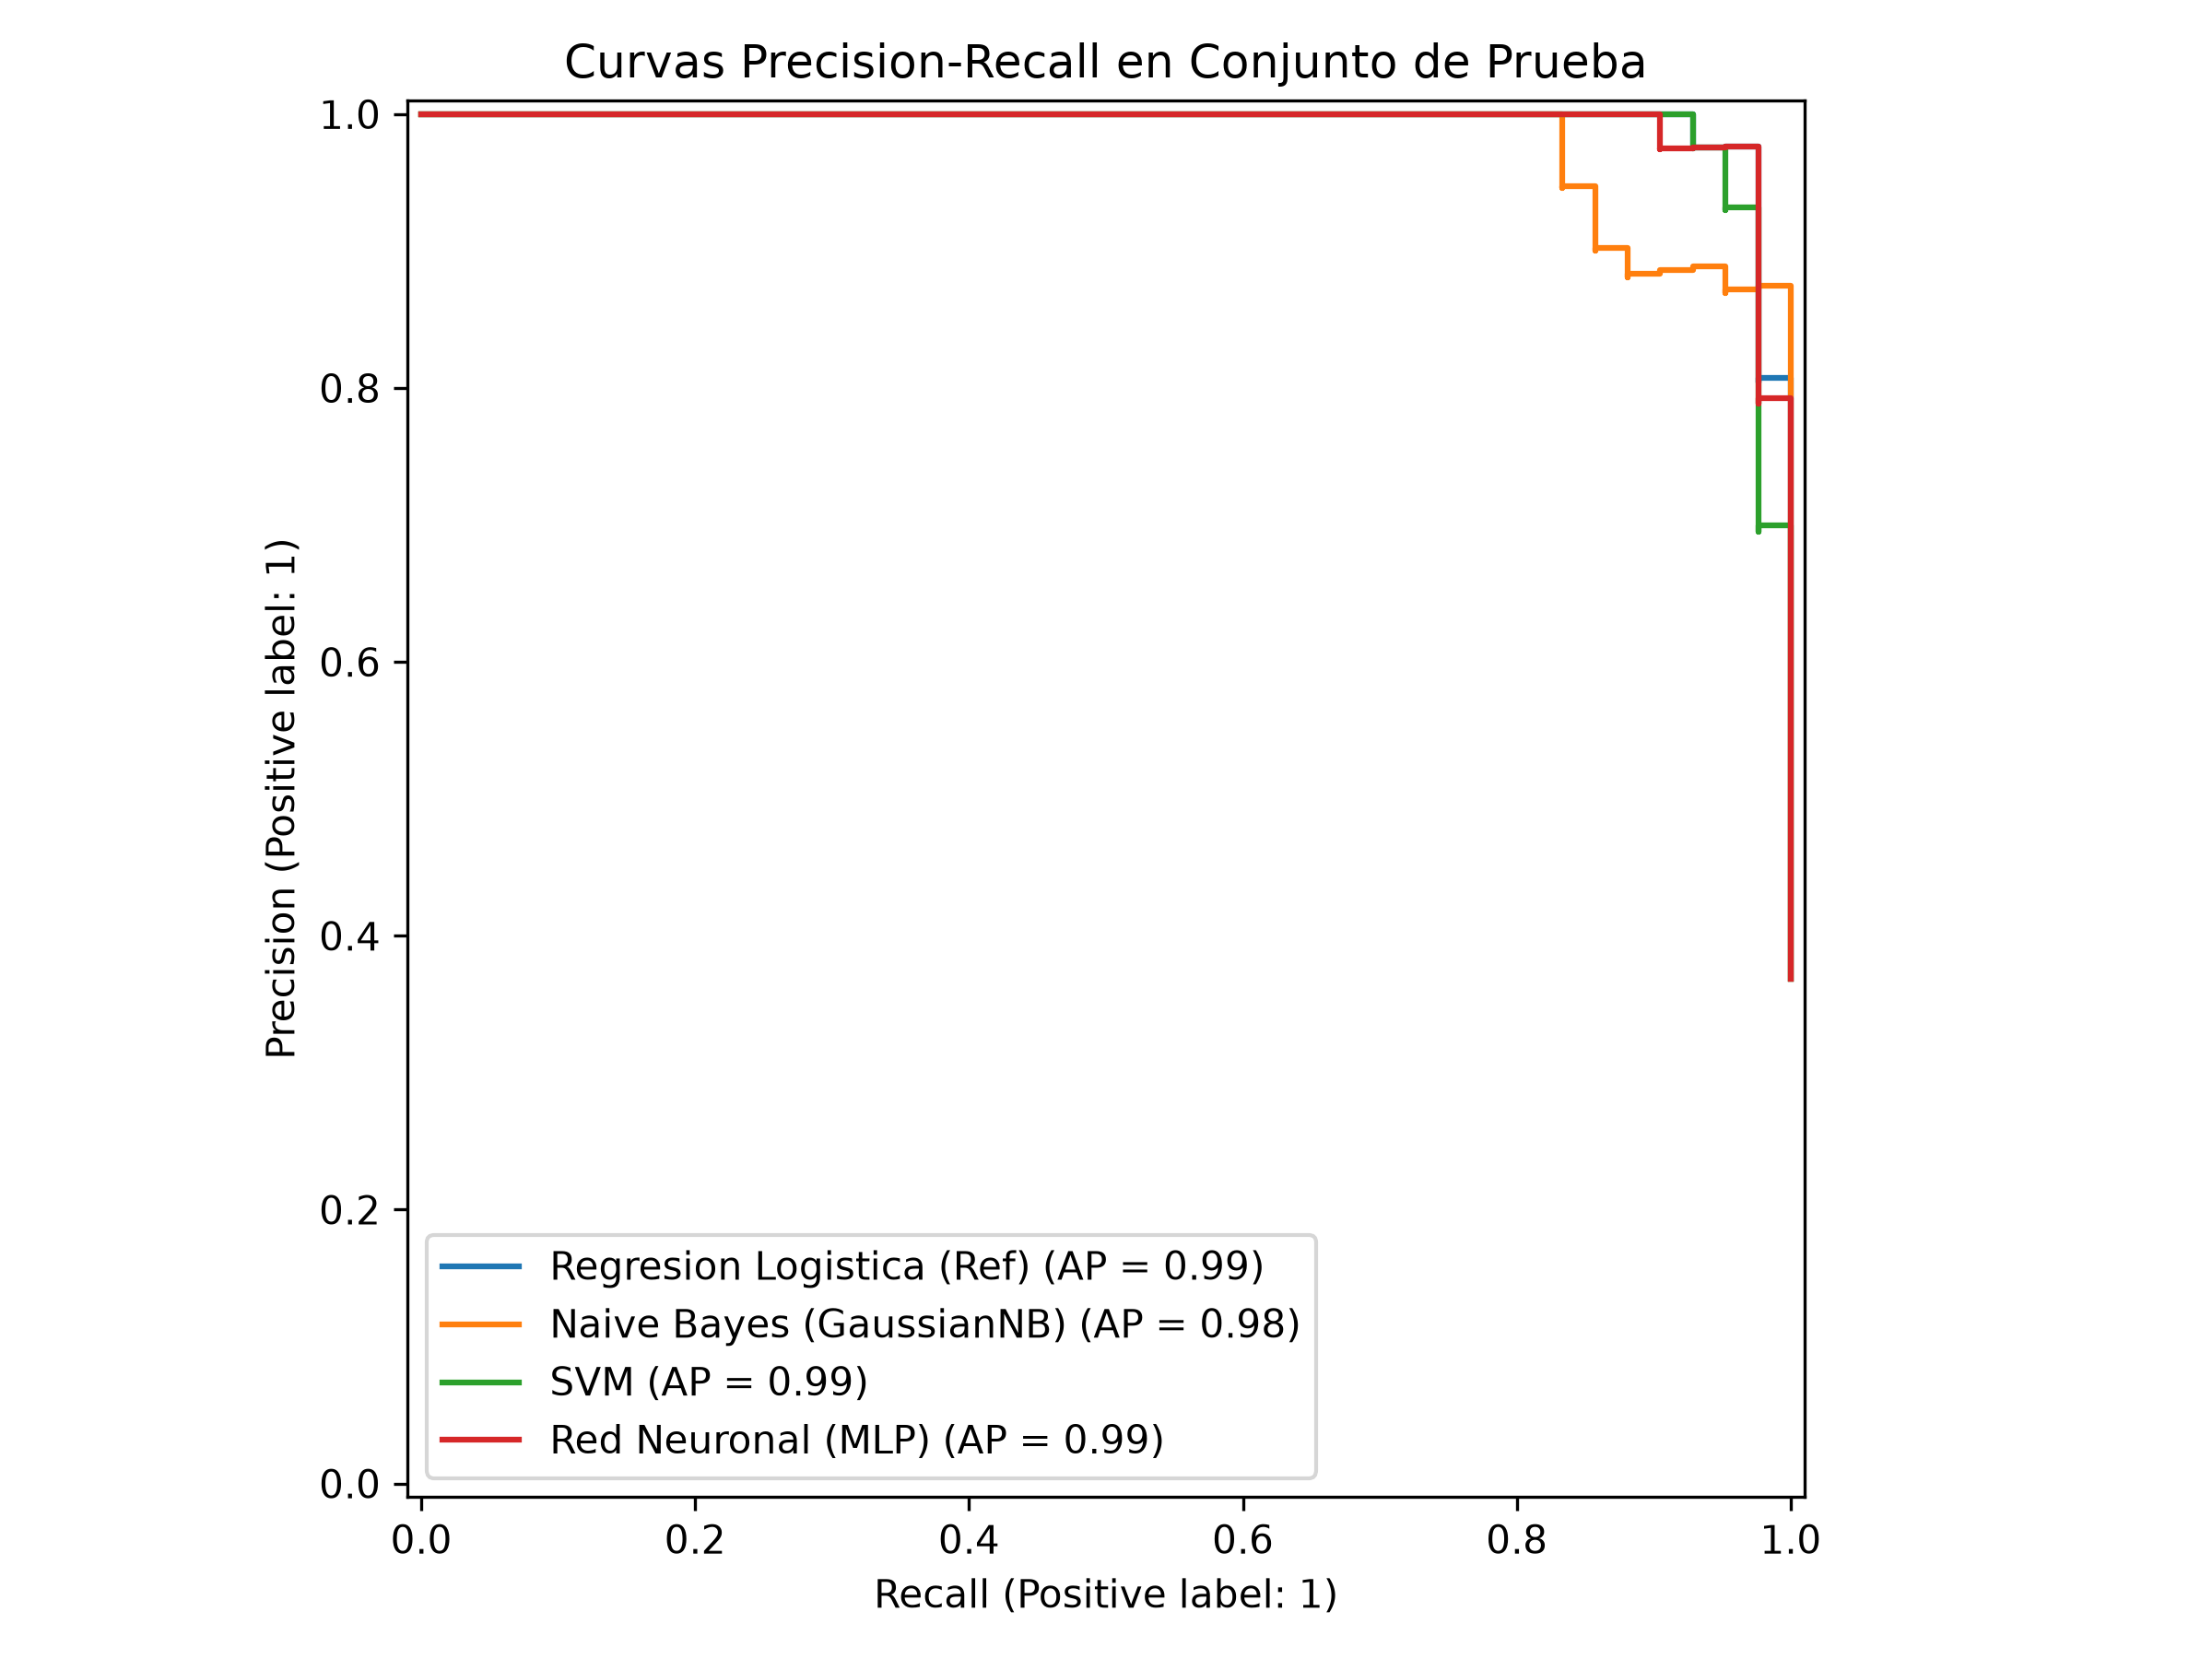
\includegraphics[width=0.92\columnwidth]{06_curvas_precision_recall}
    \caption{Curvas Precisión-Recall sobre el conjunto de prueba, evaluando el compromiso entre precisión y sensibilidad ante el desbalance moderado.}
    \label{fig:pr}
\end{figure}

\subsection{Análisis de Errores}

Al inspeccionar los registros exactos del conjunto de prueba donde falló cada algoritmo, se obtuvieron los siguientes conteos:
\begin{itemize}
    \item \textbf{Red Neuronal (MLP):} 3 errores totales (2 Falsos Negativos, 1 Falso Positivo) en los índices \texttt{[73, 208, 385]}.
    \item \textbf{SVM:} 3 errores totales (3 Falsos Negativos, 0 Falsos Positivos) en los índices \texttt{[99, 73, 205]}.
    \item \textbf{Regresión Logística (Ref):} 4 errores totales (3 Falsos Negativos, 1 Falso Positivo) en los índices \texttt{[455, 73, 190, 205]}.
    \item \textbf{Naive Bayes (GaussianNB):} 9 errores totales (6 Falsos Negativos, 3 Falsos Positivos) en los índices \texttt{[99, 318, 73, 86, 100, 505, 385, 128, 205]}.
\end{itemize}

El hallazgo más revelador del análisis de errores es que el paciente con índice \texttt{73} (diagnóstico real Maligno) fue clasificado erróneamente como Benigno por los cuatro modelos. Al revisar sus atributos, presenta \texttt{mean\_radius = 13.80}, \texttt{mean\_texture = 15.79} y \texttt{mean\_area = 584.1}, valores moderados ubicados en pleno centro de la zona de traslape de la Fig.~\ref{fig:distribucion}, donde predominan los núcleos benignos. Algo similar ocurre con los casos malignos \texttt{205} (fallado por tres modelos; \texttt{mean\_radius = 15.12}, pero textura baja de $16.68$), \texttt{99} (\texttt{mean\_radius = 14.42}) y \texttt{385} (\texttt{mean\_radius = 14.60}).

Por otro lado, los falsos positivos reflejan tumores benignos con algún rasgo atípicamente elevado: el paciente \texttt{455} (fallado por Regresión Logística) posee una textura muy alta (\texttt{mean\_texture = 30.72}), típica de casos malignos, mientras que el paciente \texttt{128} (fallado por Naive Bayes) tiene un radio y área elevados para ser benigno (\texttt{mean\_radius = 15.10}, \texttt{mean\_area = 674.5}).

\section{Discusión}

El contraste entre las métricas de validación cruzada, prueba y análisis de errores permite explicar por qué cada modelo se comportó de manera distinta:

\begin{itemize}
    \item \textbf{SVM vs. MLP y el papel de la Regresión Logística:} Aunque MLP obtuvo el mejor F1 ($0.9639$) y la mayor sensibilidad ($0.9524$) en el conjunto de prueba, SVM mostró la mayor estabilidad entre folds ($0.9674 \pm 0.0114$ frente a $0.9388 \pm 0.0140$ de MLP). Asimismo, la Regresión Logística logró $0.9640 \pm 0.0207$ en validación cruzada y el mayor ROC-AUC ($0.9960$). Dado que las desviaciones estándar de SVM y Regresión Logística se traslapan y que en una prueba de 114 pacientes un solo error cambia la exactitud en 0.88\%, la diferencia entre estos tres modelos es estrecha y confirma la separabilidad casi lineal del problema reportada en la literatura \cite{mangasarian1995}.
    \item \textbf{Impacto real de la multicolinealidad en Naive Bayes:} \texttt{GaussianNB} cometió el triple de errores que SVM y MLP (9 frente a 3) y tuvo la mayor dispersión entre folds ($\pm 0.0342$). Esto confirma experimentalmente lo anticipado en el sondeo: los 21 pares de variables con correlación superior a $0.90$ rompen el supuesto de independencia condicional, haciendo que el clasificador cuente repetidamente la misma información geométrica y genere seis falsos negativos \cite{rish2001}.
    \item \textbf{Prioridad clínica de los resultados:} En el diagnóstico de cáncer de mama, un Falso Negativo conlleva el riesgo de no tratar un tumor maligno a tiempo. Bajo este criterio clínico, la Red Neuronal MLP destaca en prueba al reducir los falsos negativos a solo 2 casos (sensibilidad de 95.24\%), mientras que SVM resulta ideal cuando se busca evitar falsas alarmas (0 falsos positivos).
\end{itemize}

\textbf{Limitaciones del estudio:} El tamaño total de la base de datos ($N = 569$) implica que el conjunto de prueba contiene únicamente 114 pacientes (42 malignos), por lo que pequeñas variaciones en la partición pueden mover las métricas en casi un punto porcentual. Además, todas las muestras provienen de una sola institución hospitalaria, por lo que los resultados no garantizan el mismo rendimiento sobre imágenes tomadas con otros equipos sin una validación externa.

\section{Conclusiones y Trabajo Futuro}

En este trabajo se aplicó un proceso completo y reproducible de ciencia de datos sobre \textit{Breast Cancer Wisconsin (Diagnostic)}, demostrando que auditar la base de datos antes de modelar permite descubrir problemas críticos como la ausencia de encabezados, los 13 ceros exactos en concavidad, las diferencias de escala y la multicolinealidad severa. El uso de \texttt{Pipeline} con estandarización y validación cruzada estratificada garantizó una evaluación justa sin fuga de información.

Los resultados demuestran que tanto SVM con kernel RBF (el más estable en validación cruzada con F1 de $0.9674 \pm 0.0114$ y precisión de $1.0000$ en prueba) como la Red Neuronal MLP de una capa oculta con activación \texttt{tanh} (mayor F1 de $0.9639$ y sensibilidad de $0.9524$ en prueba) superan ampliamente a Naive Bayes, cuya degradación se explica directamente por la violación de su supuesto de independencia. Asimismo, el sólido desempeño de la Regresión Logística ($0.9960$ en ROC-AUC) confirma que un modelo base bien regularizado sigue siendo altamente competitivo en conjuntos pequeños.

Como trabajo futuro se propone: (1) aplicar análisis de componentes principales (PCA) o selección de características para eliminar la multicolinealidad y cuantificar cuánto mejora \texttt{GaussianNB}; (2) ajustar el umbral de probabilidad por debajo de $0.5$ para intentar eliminar por completo los falsos negativos en casos frontera como el paciente \texttt{73}; y (3) validar los modelos entrenados con cohortes médicas externas.

\balance
\bibliographystyle{IEEEtran}
\bibliography{referencias}

\end{document}